% !TEX root = ../main.tex

% Gaussian process regression section

\section{Gaussian process regression} \label{section:GPs}


Gaussian process regression arises when studying functions which are computationally expensive to evaluate. The general idea is to assume that the function of interest $f$ is a stochastic process and use a sample of values of $f$ to estimate the function in unobserved values of the domain. We start by defining Gaussian processes, which are the building blocks of this idea.

\begin{definition}[Gaussian process] \label{def:GP}
	A stochastic process $X = (X_t)_{t \in \calT}$ is said to be a Gaussian process (GP) if, for any finite subset $T \subset \calT$, $X_T$ follows a Normal distribution. 
\end{definition}


\textbf{Remark.} A Gaussian process is entirely determined by its mean $m$ and covariance $\kappa$ functions. Formally, $m: t \mapsto \bbE[X_t]$ and $\kappa: (t, t') \mapsto \Cov(X_t, X_{t'})$ and we write $X \sim \GP (m, \kappa)$. Commonly, $m$ is assumed to be zero and $\kappa$ is chosen from some parametric family of functions, many of which have been thoroughly studied in the literature \cite[see][Ch.~4]{RasmussenWilliams:2006}. \\




Now we formalize GP regression. Consider a function $f: \calT \to \bbR$ and denote $X_t := f(t)$ for all $t \in \calT$. We assume that $X = (X_t) \sim \GP (m, \kappa)$. Usually, $\calT$ will be a subset of $\bbR^n$. Assuming that $m = 0$ and that we have access to observations $(X_t, t)_{t \in T}$, where $T$ is a finite subset of $\calT$, then
\begin{equation*}
	X_T \sim \calN (0, K(T, T)),
\end{equation*}
where $K$ is a $|T| \times |T|$ matrix with entries $K_{ij} = \kappa(t_i, t_j)$. If we want to predict the value of the function $f(t^{*})$, we again use the fact that
\begin{equation*}
	\begin{pmatrix} X_T \\ X_{t^{*}} \end{pmatrix} \sim \calN \left( 0, \begin{pmatrix} K(T, T) & K(T, t^{*}) \\ K(t^{*}, T) & \kappa(t^{*}, t^{*}) \end{pmatrix} \right),
\end{equation*}
from where, using basic properties of the Normal distribution,
\begin{equation} \label{eq:GPupdate}
	X_{t^{*}} \, | \, X_T \sim \calN \left( K(t^{*}, T) K(T, T)^{-1} X_T, \, \kappa(t^{*}, t^{*}) K(t^{*}, T) K(T, T)^{-1} K(T, t^{*})  \right).
\end{equation}
Commonly, the conditional mean in Equation (\ref{eq:GPupdate}) is used as a point estimate of $f(t^{*})$; the estimated variance can be used to e.g. compute confidence bands. Also, observe that we could have well chosen $t^{*}$ to have more than one component if we were interested in values of $f$ only at specific points in the covariate space. The advantage of Equation (\ref{eq:GPupdate}) is that it provides point estimates for \textit{any} point in $\calT$. Figure \ref{fig:GP1} showcases this process. \\




\begin{figure}[h]
	\centering
	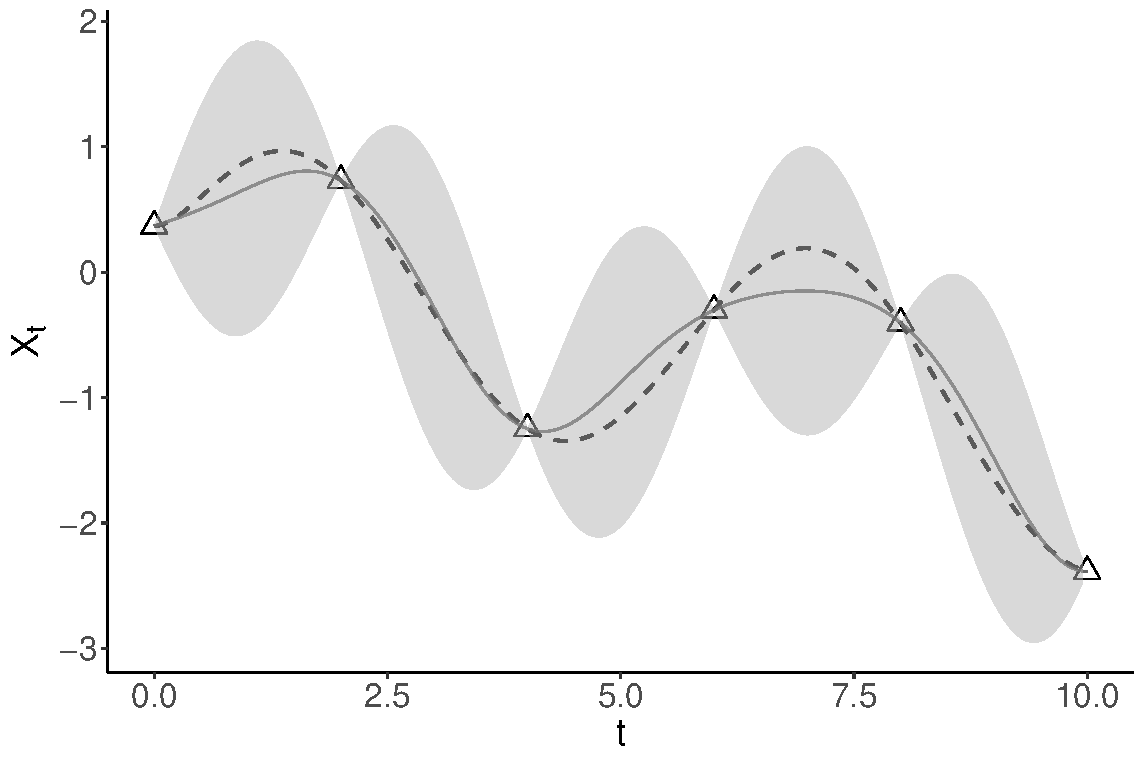
\includegraphics[scale=0.5]{GP1.pdf}
	\caption{Gaussian process regression used to estimate a function $f$ (shown in dotted grey lines). The prediction is based on the conditional mean of the GP, which is shown in a line and was fitted based on 8 observations of $f$ (the triangle shapes), along with 95\% confidence bands.}
	\label{fig:GP1}
\end{figure}



It is easy to extend this idea for cases in which, rather than having access to exact values of the function $f$, only estimates with some noise are available. This is the case, for example, when $f$ is simply impossible to evaluate, but can be reliably estimated via Monte Carlo methods---e.g. when $f$ is an expected loss over a high-dimensional parameter space. In these situations an additive noise term $\xi$ is commonly added to the covariance function $\kappa$.



% ...